\chapter{Flip flop and sequential logic}
In the first part of the experience we implemented the cicuirts: latch SR, latch SR synchronized (flip flop) and a flip flop type D. All of them by using just NAND and NOT gates. Later we built an anti-bounce latch SR and a circuit that registers an impulsive input by storing it in the memory. Later we used a J-K flip flop for building a frequency divider and a shift register. Finally we built an up-down 8-bit counter.

\section{Materials}
\begin{itemize}
\item Resistors, trimmers
\item Power supply RIGOL DP831A
\item Waveform generator RIGOL DG1032
\item Multimeter RIGOL DM3068
\item NAND 74LS00
\item NOT 74LS04
\item 74LS109
\item 74LS191
\end{itemize}
The resistors used were all with an uncertainty of 5\%

\section{Experimental setup}
We built the latch SR as in the figure \ref{SR_NAND} and for visualizing the output we  connected $Q$ and $\overline{Q}$ to an 8-led chip.
\begin{figure}[H]
\centering
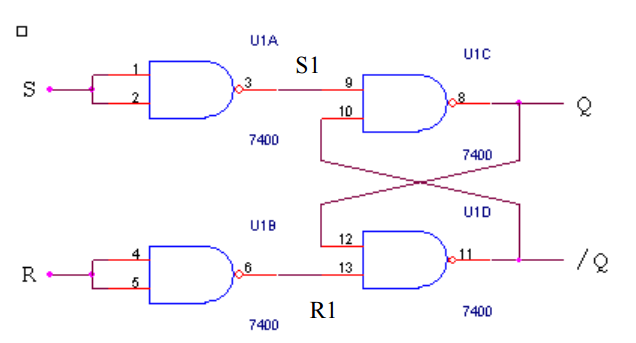
\includegraphics[width=.7\textwidth]{11/SR_NAND.png}
\caption{Latch SR}\label{SR_NAND}
\end{figure}
Later we modified the circuit as in figure \ref{FF_SR_NAND} and we verified that when EN is low voltage the circuit is in the HOLD configuration, that is it keeps the memory of the previous state. 
\begin{figure}[H]
\centering
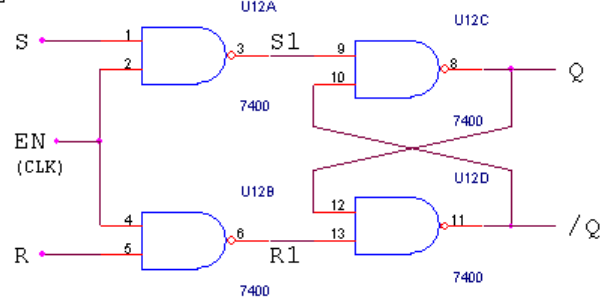
\includegraphics[width=.7\textwidth]{11/FF_SR_NAND.png}
\caption{Flip-flop built with NAND gates}\label{FF_SR_NAND}

\end{figure}
We modified again the circuit to be a FF type D (figure \ref{D_FF}) and we verified that every time the EN is on, the bit on D is registred in the memory.
\begin{figure}[H]
\centering
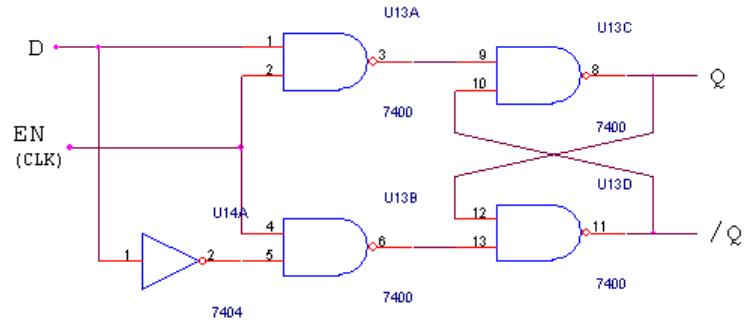
\includegraphics[width=.7\textwidth]{11/D_FF.png}
\caption{Flip flop type D}\label{D_FF}

\end{figure}

Then we  built a latch SR with an ``anti-bounce'' configuration (figure \ref{bounce}, in particular we made sure the output was changing from LOW to HIGH without too much noise.
\begin{figure}[H]
\centering
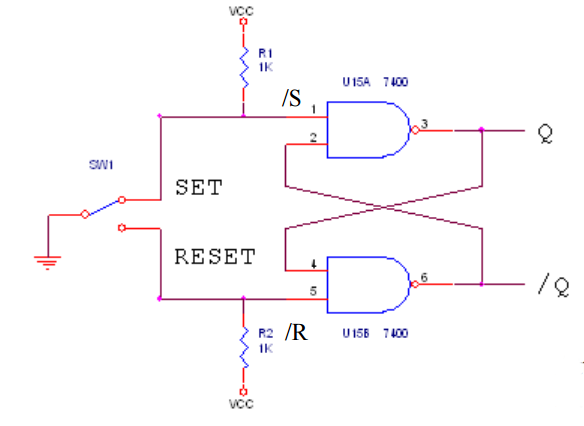
\includegraphics[width=.7\textwidth]{11/bounce.png}
\caption{Anti bounce circuit}\label{bounce}

\end{figure}
We later built an on/off system (figure \ref{ON_OFF}) that had a HIGH output when we activated SET for a short amount of time and a LOW one when we did the same with RESET.
\begin{figure}[H]
\centering
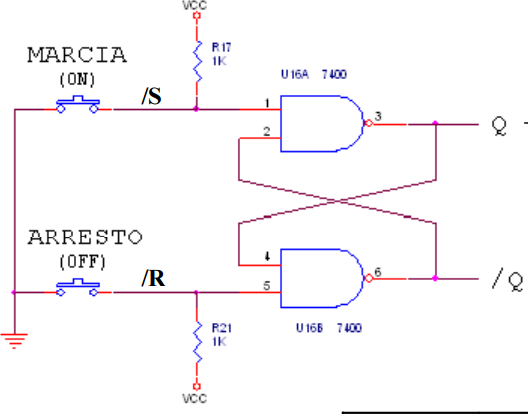
\includegraphics[width=.5\textwidth]{11/ON_OFF.png}
\caption{On-off circuit}\label{ON_OFF}

\end{figure}
We also built the frequency divider (circuit in \ref{f_div}) that gave as output a square wave with frequency that was half or a quarter of the clock, depending on where we took the output. This was done by using two J/K FF connecting the clock with the output of the previous  FF or the clock (for the first FF) and connecing J to $V_{cc}$ and K to ground. The frequency of clock used was 10 Hz.
\begin{figure}[H]
\centering
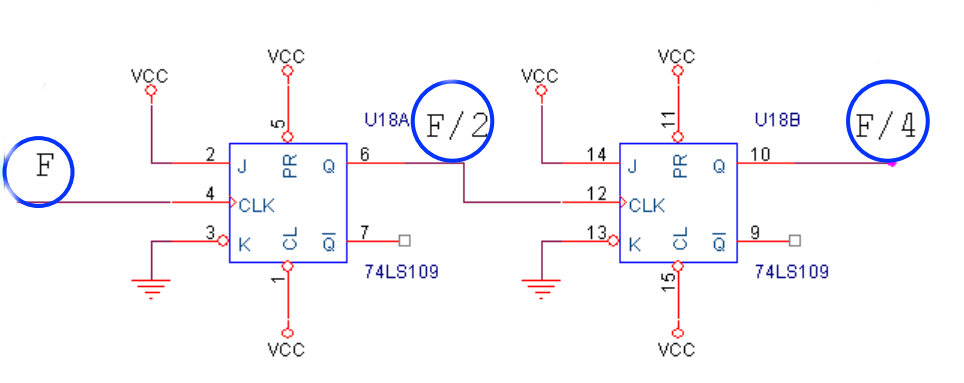
\includegraphics[width=.7\textwidth]{11/f_div.png}
\caption{Frequency divider}\label{f_div}
\end{figure}
We built the shift register in \ref{shift_reg} with four J/K FF used as FF type D. We connected the FF in circle connecting the output of one with the input of the other. We also used the pin CL and PR to preset the bit in the registers with the help of a capacitor that kept the voltage LOW for a short amount of time. We visualizied the shift register connecting the output of each FF to some LEDs.
\begin{figure}[H]
\centering
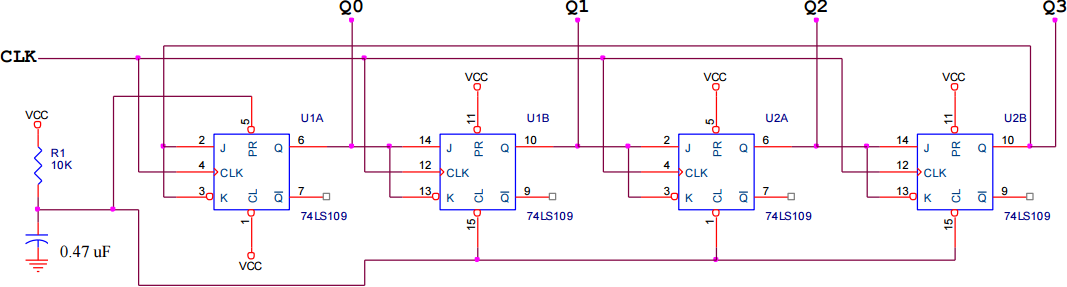
\includegraphics[width=.7\textwidth]{11/shift_reg.png}
\caption{Shift register}\label{shift_reg}

\end{figure}
At last we built a counter with two 74LS191 an a D-FF as in figure \ref{count}. The FF was used because, as stated in the 74LS191 datasheet, the up/down signal must be on the raising edge of the clock. The FF remember what we chose and transmit it to the clock when this one goes from LOW to HIGH. We used the same method used in the shift register for presetting the bits in the counter. For using an 8 bit system we needed to activate the second 74LS191 just when the bits of the first were all on, this was done by connecting RCD to G of the second one used to enable.
\begin{figure}[H]
\centering
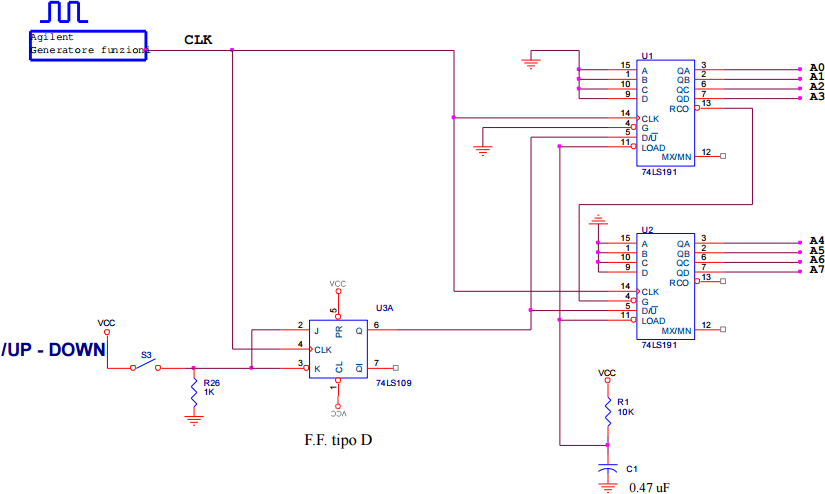
\includegraphics[width=.7\textwidth]{11/count.png}
\caption{8-bit counter}\label{count}
\end{figure}


\section{Data analysis}
We can see in the plot \ref{bounce_time} that the output of the latch SR is really noisy without the anti bounce expedient.
\begin{figure}[H]
\centering
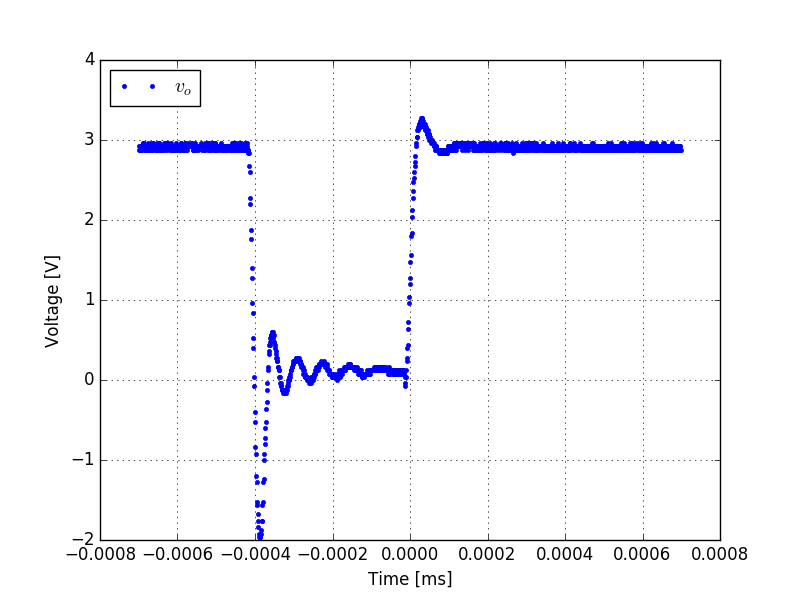
\includegraphics[width=.7\textwidth]{11/bounce_time.png}
\caption{Output of a standard latch SR}\label{bounce_time}
\end{figure}
When we modify as in \ref{bounce} we can see that the output is much more stable.
\begin{figure}[H]
\centering
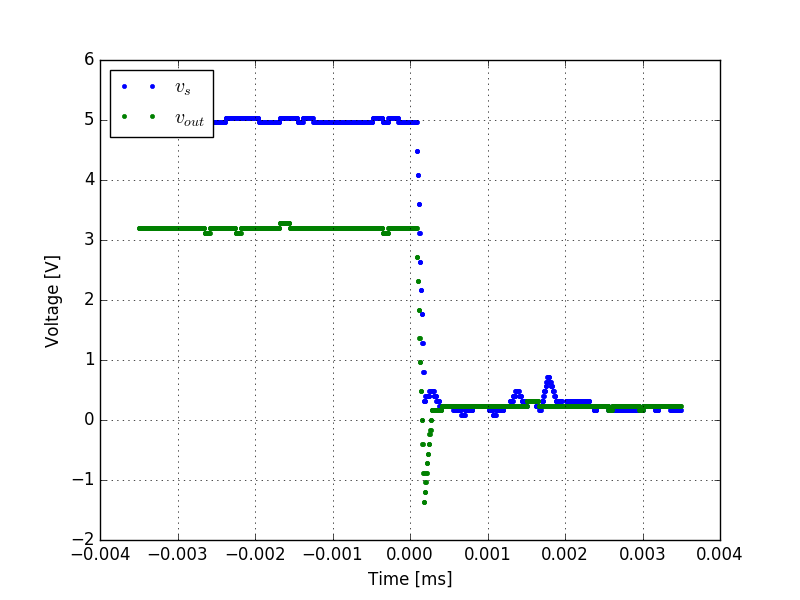
\includegraphics[width=.7\textwidth]{11/anti_bounce_time3.png}
\caption{Output of a standard latch SR}\label{anti_bounce_time3}
\end{figure}
We can see that in the plots of frequency divider circuit we have the outputs as expected with half and a quarter of the frequency of the clock.

\begin{figure}[H]
\centering
\begin{minipage}{.48\textwidth}
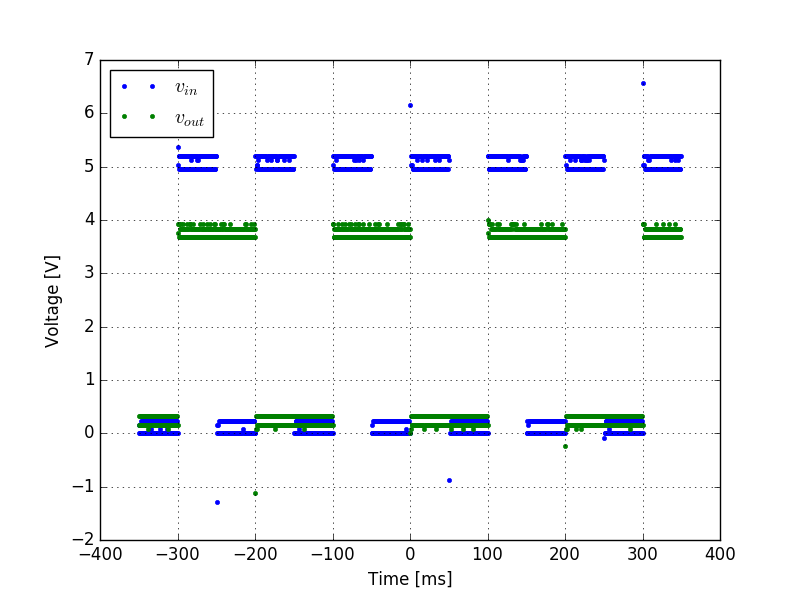
\includegraphics[width=\textwidth]{11/freq_div_m.png}
\caption{Output of frequency divider at half frequency}\label{freq_div_m}
\end{minipage}\hfill
\begin{minipage}{.48\textwidth}
\centering
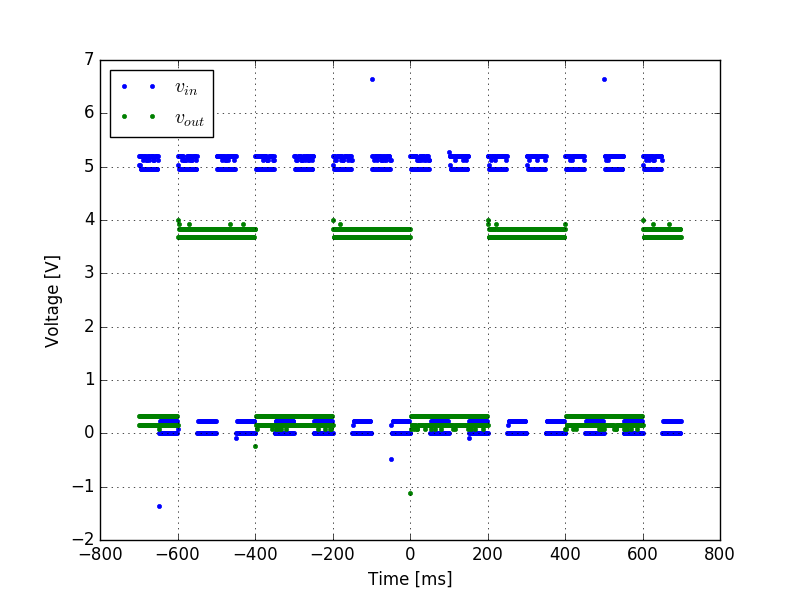
\includegraphics[width=\textwidth]{11/freq_div_q.png}
\caption{Output of frequency divider at quarter frequency}\label{freq_div_q}
\end{minipage}
\end{figure}
In the counter circuit we used a capacitor for presetting the starting bits. For this reason we measured the voltage at the capacitor's ends at the stating time and, as we expected, in the plot \ref{start_count} the voltage slowly goes to the HIGH level
\begin{figure}[H]
\centering
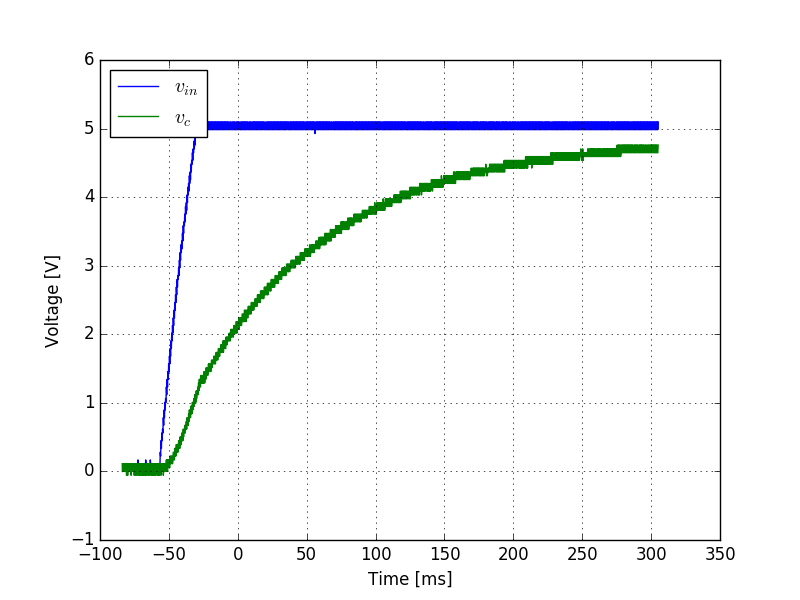
\includegraphics[width=.7\textwidth]{11/start_count.png}
\caption{In the counting circuit: the voltage of the power supply $v_{in}$ and the voltage on the ends of the capacitor $v_c$}\label{start_count}
\end{figure}
